\documentclass[a4paper,11pt]{article}

\usepackage{mlsubmit}

\begin{document}

\initmlsubmision{1}                              					% assignment number
								{Akshat Jindal}      						           		% your name
								{150075}																		% your roll number

\begin{mlsolution}


We realise that for calculating the decision boundary, the decision boundary is basically the line such that all points on the line are equidistant from the two means given to us, i.e (1,0) and (0,1) where distance is defined by the metric in the assignment.\\
\subsection*{Part1 :}
Mathematical Expression: \\
Let $\mu_{_{1}}$ be (1,0), $\mu_{_{2}}$ be (0,1). Let $\vz, \in \bR^2$ be an arbitrary point.  
\begin{equation}
    \textless(z-\mu_{_{1}} ), U(z-\mu_{_{1}})\textgreater  \ = \  \textless(z-\mu_{_{2}} ), U(z-\mu_{_{2}})\textgreater
\end{equation}
\begin{equation}
    \begin{bmatrix}
    z_{1}-1 & z_{2}
\end{bmatrix}
 \begin{bmatrix}
    3 & 0 \\
    0 & 1 
\end{bmatrix}
 \begin{bmatrix}
   z_{1}-1  \\
    z_{2}
\end{bmatrix}
=
    \begin{bmatrix}
    z_{1} & z_{2}-1
\end{bmatrix}
 \begin{bmatrix}
    3 & 0 \\
    0 & 1 
\end{bmatrix}
 \begin{bmatrix}
   z_{1}  \\
    z_{2}-1
\end{bmatrix} \\
\end{equation}
\begin{equation}
    \Rightarrow z_{2} = 3z_{1} - 1;
\end{equation} \\
\subsection*{Part2 :}
Mathematical Expression: \\
Let $\mu_{_{1}}$ be (1,0), $\mu_{_{2}}$ be (0,1). Let $\vz, \in \bR^2$ be an arbitrary point.  
\begin{equation}
    \textless(z-\mu_{_{1}} ), U(z-\mu_{_{1}})\textgreater  \ = \  \textless(z-\mu_{_{2}} ), U(z-\mu_{_{2}})\textgreater
\end{equation}
\begin{equation}
    \begin{bmatrix}
    z_{1}-1 & z_{2}
\end{bmatrix}
 \begin{bmatrix}
    1 & 0 \\
    0 & 0 
\end{bmatrix}
 \begin{bmatrix}
   z_{1}-1  \\
    z_{2}
\end{bmatrix}
=
    \begin{bmatrix}
    z_{1} & z_{2}-1
\end{bmatrix}
 \begin{bmatrix}
    1 & 0 \\
    0 & 0 
\end{bmatrix}
 \begin{bmatrix}
   z_{1}  \\
    z_{2}-1
\end{bmatrix} \\
\end{equation}
\begin{equation}
    \Rightarrow z_{1} = 1/2;
\end{equation} \\
\begin{figure}[th]%
\centering
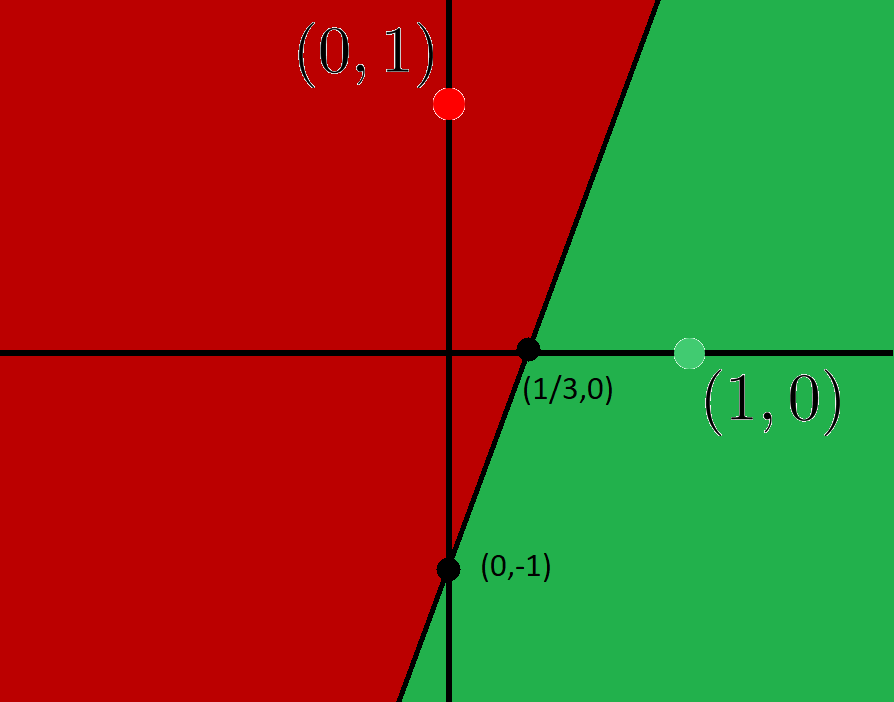
\includegraphics[width=0.3\columnwidth]{Part1.png}%
\hfill
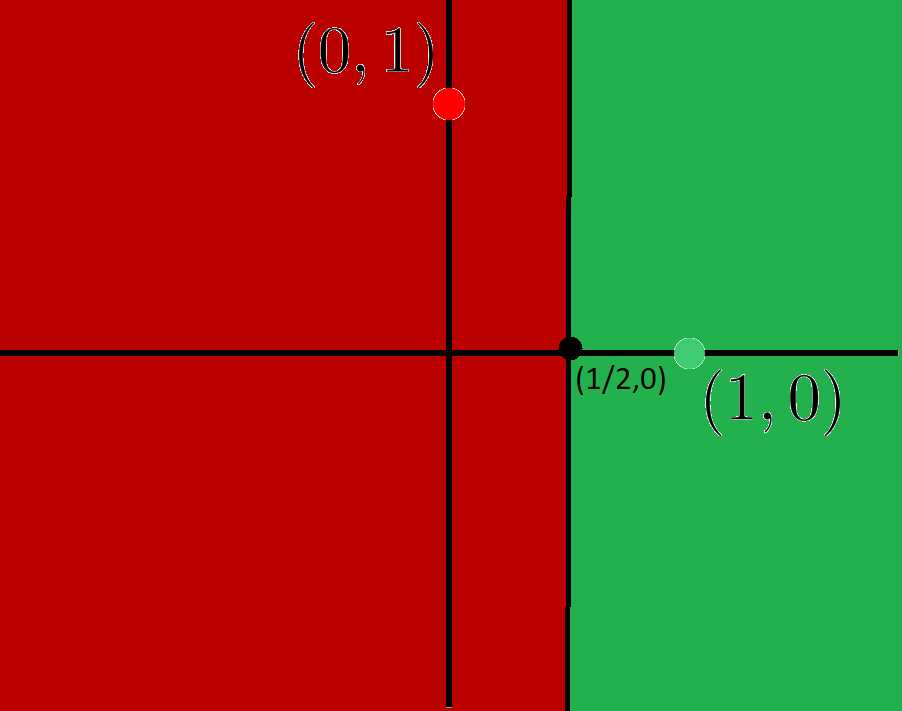
\includegraphics[width=0.3\columnwidth]{Part2.png}%
\caption{Learning with Prototypes: Left figure is for Part 1, right figure is for Part 2}%
\label{fig:proto}%
\end{figure}

\end{mlsolution}

\begin{mlsolution}
\subsection*{Designing the Likelihood}
Before beginning with the solution, we make the assumption that the training data points given to us are i.i.d Random Variables. This allows us to express the probability of the response vector $ y \in \bR^d$ as the product of the probability of the individual responses. i.e : 
\begin{equation}
    P(y|X,w) =  \prod_{i=1}^{n} P(y^i|x^i,w)
\end{equation}
Since we only have to model the responses, we deal with conditional probabilities only.We know from previous experience in the class that the given loss function term arises from a Gaussian Likelihood with mean = $\textless w,x \textgreater$. \\
\\
Thus, for any constant $\sigma$:
\begin{equation}
y^i \sim N(<w,x^i>,\sigma ^2)  
\end{equation}
For k as a constant:
\begin{align}
    P(y|X,w) &=  \prod_{i=1}^{n} P(y^i|x^i,w)\\
    P(y|X,w) &=  \prod_{i=1}^{n} k * e^{-(y^i - <w,x^i>)^2/(2\sigma^2)}\\
\end{align}
Taking log both sides, the Negative Likelihood Objective becomes:
\begin{align}
    NLL(w) &=  1/2\sigma^2 * \sum_{i=1}^{n}((y^i - <w,x^i>)^2)
\end{align}
\subsection*{Designing the Prior Distribution}
This designing can be thought of as very intuitive. Since our feasible region is only thos $w$ such that their $l_{2}$ norm $\leqslant \ r$, we come up with this distribution: \\
\abovedisplayskip=0pt\relax
\[
 P(w) =
\left\{
\!
\begin{aligned}
\alpha & \text{ if } \norm{w}_{2} \leqslant \ r\\
0 & \text{ if } o.w\\
\end{aligned}
\right.
\]

To make the above a legal probability distro, $\alpha$ is such that $\int_{w}\alpha = 1 \ \forall w$ \ such that $\norm{w}_{2} \leqslant \ r$ . Let's calculate the MAP estimate to show that this indeed works.
\subsection*{The MAP estimate}
\begin{align}
    P(w|X,y) &= (P(y|X,w) * P(w))/P(y)
\end{align}
Thus clearly:
\begin{align}
    &MAP \ Objective = MLE \ Objective + \log{P(w)}\\
    &Negative \ MAP \ Objective = NLL(w) - \log{P(w)}\\
    &\hat{w_{MAP}} = argmin \{ NLL(w) - \log{P(w)}\}\\ 
\end{align}
\subsubsection*{Explanation}
Looking at Equation 17, we see that because of the way in which P(w) is defined, $\forall$ $w$(s) s.t $\norm{w}_{2} \textgreater \ r$, P(w) becomes 0. This causes the $\log{P(w)}$ term to tend to $- \infty$. This causes the Negative MAP Objective to tend to $+ \infty$ and thus such $w$(s) will never serve as potential candidates for $\hat{w_{MAP}}$. As for the $w$(s) s.t $\norm{w}_{2} \leqslant \ r$, the $\log{P(w)}$ term is a constant and the $\hat{w_{MAP}}$ essentially becomes $\hat{w_{MLE}}$. Thus this designing of Likelihood and Prior will lead to the same optimisation problem :)  

\end{mlsolution}

\begin{mlsolution}
Before beginning, we set up the following notation for the objective function:
\begin{align}
    L(w) = \sum_{i=1}^{n}((y^i - <w,x^i>)^2) + \sum_{j=1}^{n} \alpha_{j}(w_{j}^2) 
\end{align}

\subsection*{Designing the Likelihood}
We make the assumption that the training data points given to us are i.i.d Random Variables. This allows us to express the probability of the response vector $ y \in \bR^d$ as the product of the probability of the individual responses. i.e : 
\begin{equation}
    P(y|X,w) =  \prod_{i=1}^{n} P(y^i|x^i,w)
\end{equation}
Since we only have to model the responses, we deal with conditional probabilities only.We know from previous experience in the class that the given loss function term arises from a Gaussian Likelihood with mean = $\textless w,x \textgreater$. \\
\\
Thus, for any constant $\sigma$:
\begin{equation}
y^i \sim N(<w,x^i>,\sigma ^2)  
\end{equation}
For k as any constant:
\begin{align}
    P(y|X,w) &=  \prod_{i=1}^{n} P(y^i|x^i,w)\\
    P(y|X,w) &=  \prod_{i=1}^{n} k * e^{-(y^i - <w,x^i>)^2/(2\sigma^2)}\\
\end{align}
Taking log both sides, the Negative Likelihood Objective becomes:
\begin{align}
    NLL(w) &=  1/2\sigma^2 * \sum_{i=1}^{n}((y^i - <w,x^i>)^2)
\end{align}

\subsection*{Designing the prior}
Now, we need to create a prior which will lead to the \emph{feature-regularized} regularization term. We propose that $w \sim$ A MultiVariate Gaussian Distribution with mean = $0 \in \bR^d$ and $\sum$ as the Covariance matrix:
\begin{align}
    w \sim N(0,\sum)
\end{align}
Where, $\sum$ is the following diagonal co-variance matrix: \\
\[
  D =
  \begin{bmatrix}
    (\beta_{1})^{-1} & & \\
    & \ddots & \\
    & & (\beta_{d})^{-1}
  \end{bmatrix}
\]
Thus, for k as any constant:\\
\begin{align}
    P(w) = k*e^{\frac{-(w^T.\sum^{-1}.w)}{2}}
\end{align}

\subsection*{The MAP estimate}
\begin{align}
    P(w|X,y) &= (P(y|X,w) * P(w))/P(y)
\end{align}
Thus clearly:
\begin{align}
    &MAP \ Objective = MLE \ Objective + \log{P(w)}\\
    &\Rightarrow \hat{w_{MAP}} = argmax\{ \  -1/2\sigma^2 * \sum_{i=1}^{n}((y^i - < w,x^i >)^2) + \log{k*e^{\frac{-(w^T.\sum^{-1}.w)}{2}}}\}\\
    &\Rightarrow \hat{w_{MAP}} = argmax\{ \  -1/2\sigma^2 * \sum_{i=1}^{n}((y^i - < w,x^i >)^2) - {\frac{(w^T.\sum^{-1}.w)}{2}}\}\\
    &\Rightarrow \hat{w_{MAP}} = argmax\{ \  -1/2\sigma^2 * \sum_{i=1}^{n}((y^i - < w,x^i >)^2) - \sum_{i=1}^{d}\frac{{}\beta_{i}w_{i}^2}{2}\}\\
\end{align}
Stowing away the constants into $\beta_{i}$ terms, and removing the minus sign overall: \\
\begin{align}
    &\hat{w}_{MAP} = argmin\{ \ \sum_{i=1}^{n}((y^i - < w,x^i >)^2) + \sum_{i=1}^{d} \alpha_{i}w_{i}^2\}\\
\end{align}
Thus, the map estimate $\hat{w_{fr}}$(mentioned in question) is the map estimate of our model.

\subsection*{Closed form solution}
\begin{align}
    L(w) &= \sum_{i=1}^{n}((y^i - <w,x^i>)^2) + \sum_{j=1}^{n} \alpha_{j}(w_{j}^2)\\
    \nabla (L(w)) &= 2* \sum_{i=1}^{n}(y^i - <w,x^i>)\nabla (y^i - <w,x^i>) + \nabla \sum_{j=1}^{n} \alpha_{j}(w_{j}^2) \\
    \nabla (L(w)) &= 2* \sum_{i=1}^{n}(y^i - <w,x^i>)(-x^i) + \nabla \sum_{j=1}^{n} \alpha_{j}(w_{j}^2)
\end{align}
Let's call A: \\
\[
  A =
  \begin{bmatrix}
    (\alpha_{1})^{-1} & & \\
    & \ddots & \\
    & & (\alpha_{d})^{-1}
  \end{bmatrix}
\]
Also, we call X as the design matrix, i.e X is an N x D matrix, one column for each feature. Putting $\nabla (L(w)) = 0$, we get: \\
\begin{align}
    X^Ty &= X^TXw + Aw\\
    \Rightarrow w &= (X^TX + A)^{-1}X^Ty
\end{align}
Thus derived.\\
\qed
 
\end{mlsolution}

\begin{mlsolution}
We knoe the Crammer-Singer formulation $(P1)$ for a single machine learner for multi-classification is
\begin{align*}
\bc{\widehat\vW, \{\hat\xi_i\}} = \underset{\vW,\bc{\xi_i}}{\arg\min}&\ \sum_{k=1}^K\norm{\vw^k}_2^2 + \sum_{i=1}^n\xi_i\\
\text{s.t.} &\ \ip{\vw^{y^i}}{\vx^i} \geq \ip{\vw^k}{\vx^i} + 1 - \xi_i, \forall i, \forall k \neq y^i\qquad\qquad{(P1)}\\
&\ \xi_i \geq 0, \text{ for all } i
\end{align*}
On the other hand, (P2) is :
	\[
	\phantom{\hspace{20ex}}\widehat\vW = \underset{\vW}{\arg\min}\ \sum_{k=1}^K\norm{\vw^k}_2^2 + \sum_{i=1}^n\ell_\text{cs}(y^i,\veta^i)\qquad\qquad{(P2)},
	\]
	where $\veta^i = \ip{\vW}{\vx^i}$ and
	\[
	\ell_\text{cs}(y^i,\veta^i) = [1 + \max_{k \neq y}\veta^i_k - \veta^i_y]_+
	\]
We shuffle around the constraint conditions of (P1) as follows: \\
\begin{align*}
   &\ip{\vw^{y^i}}{\vx^i} \geq \ip{\vw^k}{\vx^i} + 1 - \xi_i, \forall i, \forall k \neq y^i \\
   &\Rightarrow \xi_i \geq 1 + \ip{\vw^k}{\vx^i} - \ip{\vw^{y^i}}{\vx^i} \forall i, \forall k \neq y^i \\
   &\Rightarrow \xi_i \geq 1 + \veta^i_k - \veta^i_y \ \ \forall i, \forall k \neq y^i \\
   &\Rightarrow \xi_i \geq 1 + \max_{k \neq y}\veta^i_k - \veta^i_y \ \ \forall i \\
\end{align*}
But we know, that $\xi_i \geq 0, \text{ for all } i$, thus
\begin{align*}
   &\Rightarrow \xi_i \geq \max\{1 + \max_{k \neq y}\veta^i_k - \veta^i_y , 0 \} \ \ \forall i \\
\end{align*}
But this means:
\abovedisplayskip=0pt\relax
\[
  \xi_i >=
\left\{
\!
\begin{aligned}
&0   \ \ \ \ \ \ \ \ \ \ \ \ \ \ \ \ \  \ \text{ if } \veta^i_y - \max_{k \neq y}\veta^i_k > 1\\
&1 + \max_{k \neq y}\veta^i_k - \veta^i_y  \ \ \ o.w\\
\end{aligned}
\right.
\]
Which implies that: $\xi_i >= \ell_\text{cs}(y^i,\veta^i) = [1 + \max_{k \neq y}\veta^i_k - \veta^i_y]_+$ \\
So, we can rewrite (P1) as :
\begin{align*}
\bc{\widehat\vW, \{\hat\xi_i\}} = \underset{\vW,\bc{\xi_i}}{\arg\min}&\ \sum_{k=1}^K\norm{\vw^k}_2^2 + \sum_{i=1}^n\xi_i\\
\text{s.t.} &\ \xi_i >= \ell_\text{cs}(y^i,\veta^i) = [1 + \max_{k \neq y}\veta^i_k - \veta^i_y]_+ \forall i \qquad\qquad{(P1)}\\
\end{align*}
Now realize that since we want to minimise our objective function, in any optimal solution $\bc{\vW^0, \{\xi^0_i\}}$ for $(P_1)$,  $\xi^0_i = \ell_\text{cs}(y^i,\veta^i) = [1 + \max_{k \neq y}\veta^i_k - \veta^i_y]_+ \ \forall i$ \\


This is because if we take any $\xi^1_i > \ell_\text{cs}(y^i,\veta^i) = [1 + \max_{k \neq y}\veta^i_k - \veta^i_y]_+ \ \forall i$, then we can replace  $\xi^1_i \ \forall i$ by $\xi^0_i$ in the objective function to squeeze down $\sum_{k=1}^K\norm{\vw^k}_2^2 + \sum_{i=1}^n\xi^1_i$ to $\sum_{k=1}^K\norm{\vw^k}_2^2 + \sum_{i=1}^n\xi^0_i$ \\ \\
Thus, no matter what $\bc{\vW^0}$ you get, the $\xi^0_i$ will always be $\ell_\text{cs}(y^i,\veta^i) = [1 + \max_{k \neq y}\veta^i_k - \veta^i_y]_+ \ \forall i$. Thus solving P1 is equivalent to solving :
\[
	\phantom{\hspace{20ex}}\widehat\vW = \underset{\vW}{\arg\min}\ \sum_{k=1}^K\norm{\vw^k}_2^2 + \sum_{i=1}^n[1 + \max_{k \neq y}\veta^i_k - \veta^i_y]_+
	\]
which is essentially P2 only.\\
Thus both the optimization problems are infact the same.\\
\qed

\end{mlsolution}


\begin{mlsolution}
\subsection*{Aim}
To show that $g$ is a member of the subdifferentials of $f$ at $w$. i.e. \\ 
To prove $\forall w^{'} \in \bR^d$ : $f(w^{'}) \ - f(w) \geq \langle g, w^{'} - w \rangle$ \\
We will prove this inequality by proving it for 1 arbitrary $ \ i \in [1,N]$ and then putting summation sign on both sides of the equation.\\
Thus, our objective becomes proving, for arbitrary $w^{'} \in \bR^d$:
\begin{align}
    [1-y^{i}\langle w^{'},x^i \rangle ]_{+} - [1-y^{i}\langle w,x^i \rangle ]_{+} \geq \langle h^i, w^{'} - w \rangle
\end{align}

For convenience, we define the function $\forall a,b \in \bR$:
\[
 [1-a.b]_{+} =
\left\{
\!
\begin{aligned}
0 & \text{ if } a.b \geq 1\\
1-a.b & \text{ if } a.b < 1\\
\end{aligned}
\right.
\]

\subsection*{Case 1: $y^{i}\langle w,x^i \rangle \geq 1$}
\subsubsection*{Subcase A: $y^{i}\langle w^{'},x^i \rangle \geq 1$}

\textbf{LHS:} 
\begin{align}
    &[1-y^{i}\langle w^{'},x^i \rangle ]_{+} - [1-y^{i}\langle w,x^i \rangle ]_{+} \\
    &= 0 - 0 \ ( \ by \ definition \ above \ ) \\
    &=0
\end{align}
\textbf{RHS:}
\begin{align}
     &\langle h^i, w^{'} - w \rangle\\
    &= 0  \ ( \ by \ definition \ of \ h^i \ )
\end{align}
Thus, LHS \textgreater= RHS.

\subsubsection*{Subcase B: $y^{i}\langle w^{'},x^i \rangle < 1$}

\textbf{LHS:} 
\begin{align}
    &[1-y^{i}\langle w^{'},x^i \rangle ]_{+} - [1-y^{i}\langle w,x^i \rangle ]_{+} \\
    &= 1-y^{i}\langle w^{'},x^i \rangle - 0 \ ( \ by \ definition \ above \ ) \\
\end{align}
Note: LHS \textgreater \ 0 as $y^{i}\langle w^{'},x^i \rangle < 1$\\
\textbf{RHS:}
\begin{align}
     &\langle h^i, w^{'} - w \rangle\\
    &= 0  \ ( \ by \ definition \ of \ h^i \ )
\end{align}
Thus, LHS \textgreater  = RHS.

\subsection*{Case 2: $y^{i}\langle w,x^i \rangle < \  1$}
\subsubsection*{Subcase A: $y^{i}\langle w^{'},x^i \rangle \geq 1$}

\textbf{LHS:} 
\begin{align}
    &[1-y^{i}\langle w^{'},x^i \rangle ]_{+} - [1-y^{i}\langle w,x^i \rangle ]_{+} \\
    &= 0 - (1-y^{i}\langle w,x^i \rangle) \ ( \ by \ definition \ above \ ) \\
    &= y^{i}\langle w,x^i \rangle - 1
\end{align}
\textbf{RHS:}
\begin{align}
     &\langle h^i, w^{'} - w \rangle\\
    &= \langle -y^ix^i, w^{'} - w \rangle  \ ( \ by \ definition \ of \ h^i \ )\\
    &= y^{i}\langle x^i,w \rangle - y^{i}\langle x^i,w^{'} \rangle \ [ \ y^i \ is \ constant \ and \ dot \ product \ can \ be \ split \ ] \\
    &= y^{i}\langle w,x^i \rangle - y^{i}\langle w^{'},x^i \rangle
\end{align}
So, we observe: \\
\begin{align}
    &y^{i}\langle w^{'},x^i \rangle \geq 1 \ [We \ are \ in \ subcase \ A]\\
    &\Rightarrow -y^{i}\langle w^{'},x^i \rangle <=  -1\\
    &\Rightarrow  y^{i}\langle w,x^i \rangle - y^{i}\langle w^{'},x^i \rangle <= y^{i}\langle w,x^i \rangle - 1\\
    &\Rightarrow RHS <= LHS
\end{align}
Thus, LHS \textgreater =  RHS.

\subsubsection*{Subcase B: $y^{i}\langle w^{'},x^i \rangle < 1$}

\textbf{LHS:} 
\begin{align}
    &[1-y^{i}\langle w^{'},x^i \rangle ]_{+} - [1-y^{i}\langle w,x^i \rangle ]_{+} \\
    &= y^{i}\langle w,x^i \rangle - y^{i}\langle w^{'},x^i \rangle \ ( \ by \ definition \ above \ ) \\
\end{align}
\textbf{RHS:}
\begin{align}
     &\langle h^i, w^{'} - w \rangle\\
    &= y^{i}\langle x^i,w \rangle - y^{i}\langle x^i,w^{'} \rangle  \ ( \ by \ definition \ of \ h^i \ )\\
    &= y^{i}\langle w,x^i \rangle - y^{i}\langle w^{'},x^i \rangle
\end{align}
Thus, LHS \textgreater =  RHS.\\
Thus, for all cases, we proved that :
\begin{align}
    [1-y^{i}\langle w^{'},x^i \rangle ]_{+} - [1-y^{i}\langle w,x^i \rangle ]_{+} \geq \langle h^i, w^{'} - w \rangle
\end{align}
Thus: \\
\begin{align}
    &\sum_{i=1}^{n}[1-y^{i}\langle w^{'},x^i \rangle ]_{+} - \sum_{i=1}^{n}[1-y^{i}\langle w,x^i \rangle ]_{+} \geq \sum_{i=1}^{n}\langle h^i, w^{'} - w \rangle \\
    &\sum_{i=1}^{n}[1-y^{i}\langle w^{'},x^i \rangle ]_{+} - \sum_{i=1}^{n}[1-y^{i}\langle w,x^i \rangle ]_{+} \geq \langle \sum_{i=1}^{n}h^i, w^{'} - w \rangle \\
    &\sum_{i=1}^{n}[1-y^{i}\langle w^{'},x^i \rangle ]_{+} - \sum_{i=1}^{n}[1-y^{i}\langle w,x^i \rangle ]_{+} \geq \langle g, w^{'} - w \rangle \\
    &f(w^{'}) \ - f(w) \geq \langle g, w^{'} - w \rangle
\end{align}
Since the $w^{'}$ we chose was arbitrary, the result has been proven $\forall w^{'} \in \bR^d$\\
\qed
\end{mlsolution}
			
\begin{mlsolution}
\subsection*{Part1}
\begin{figure}[th]%
\centering
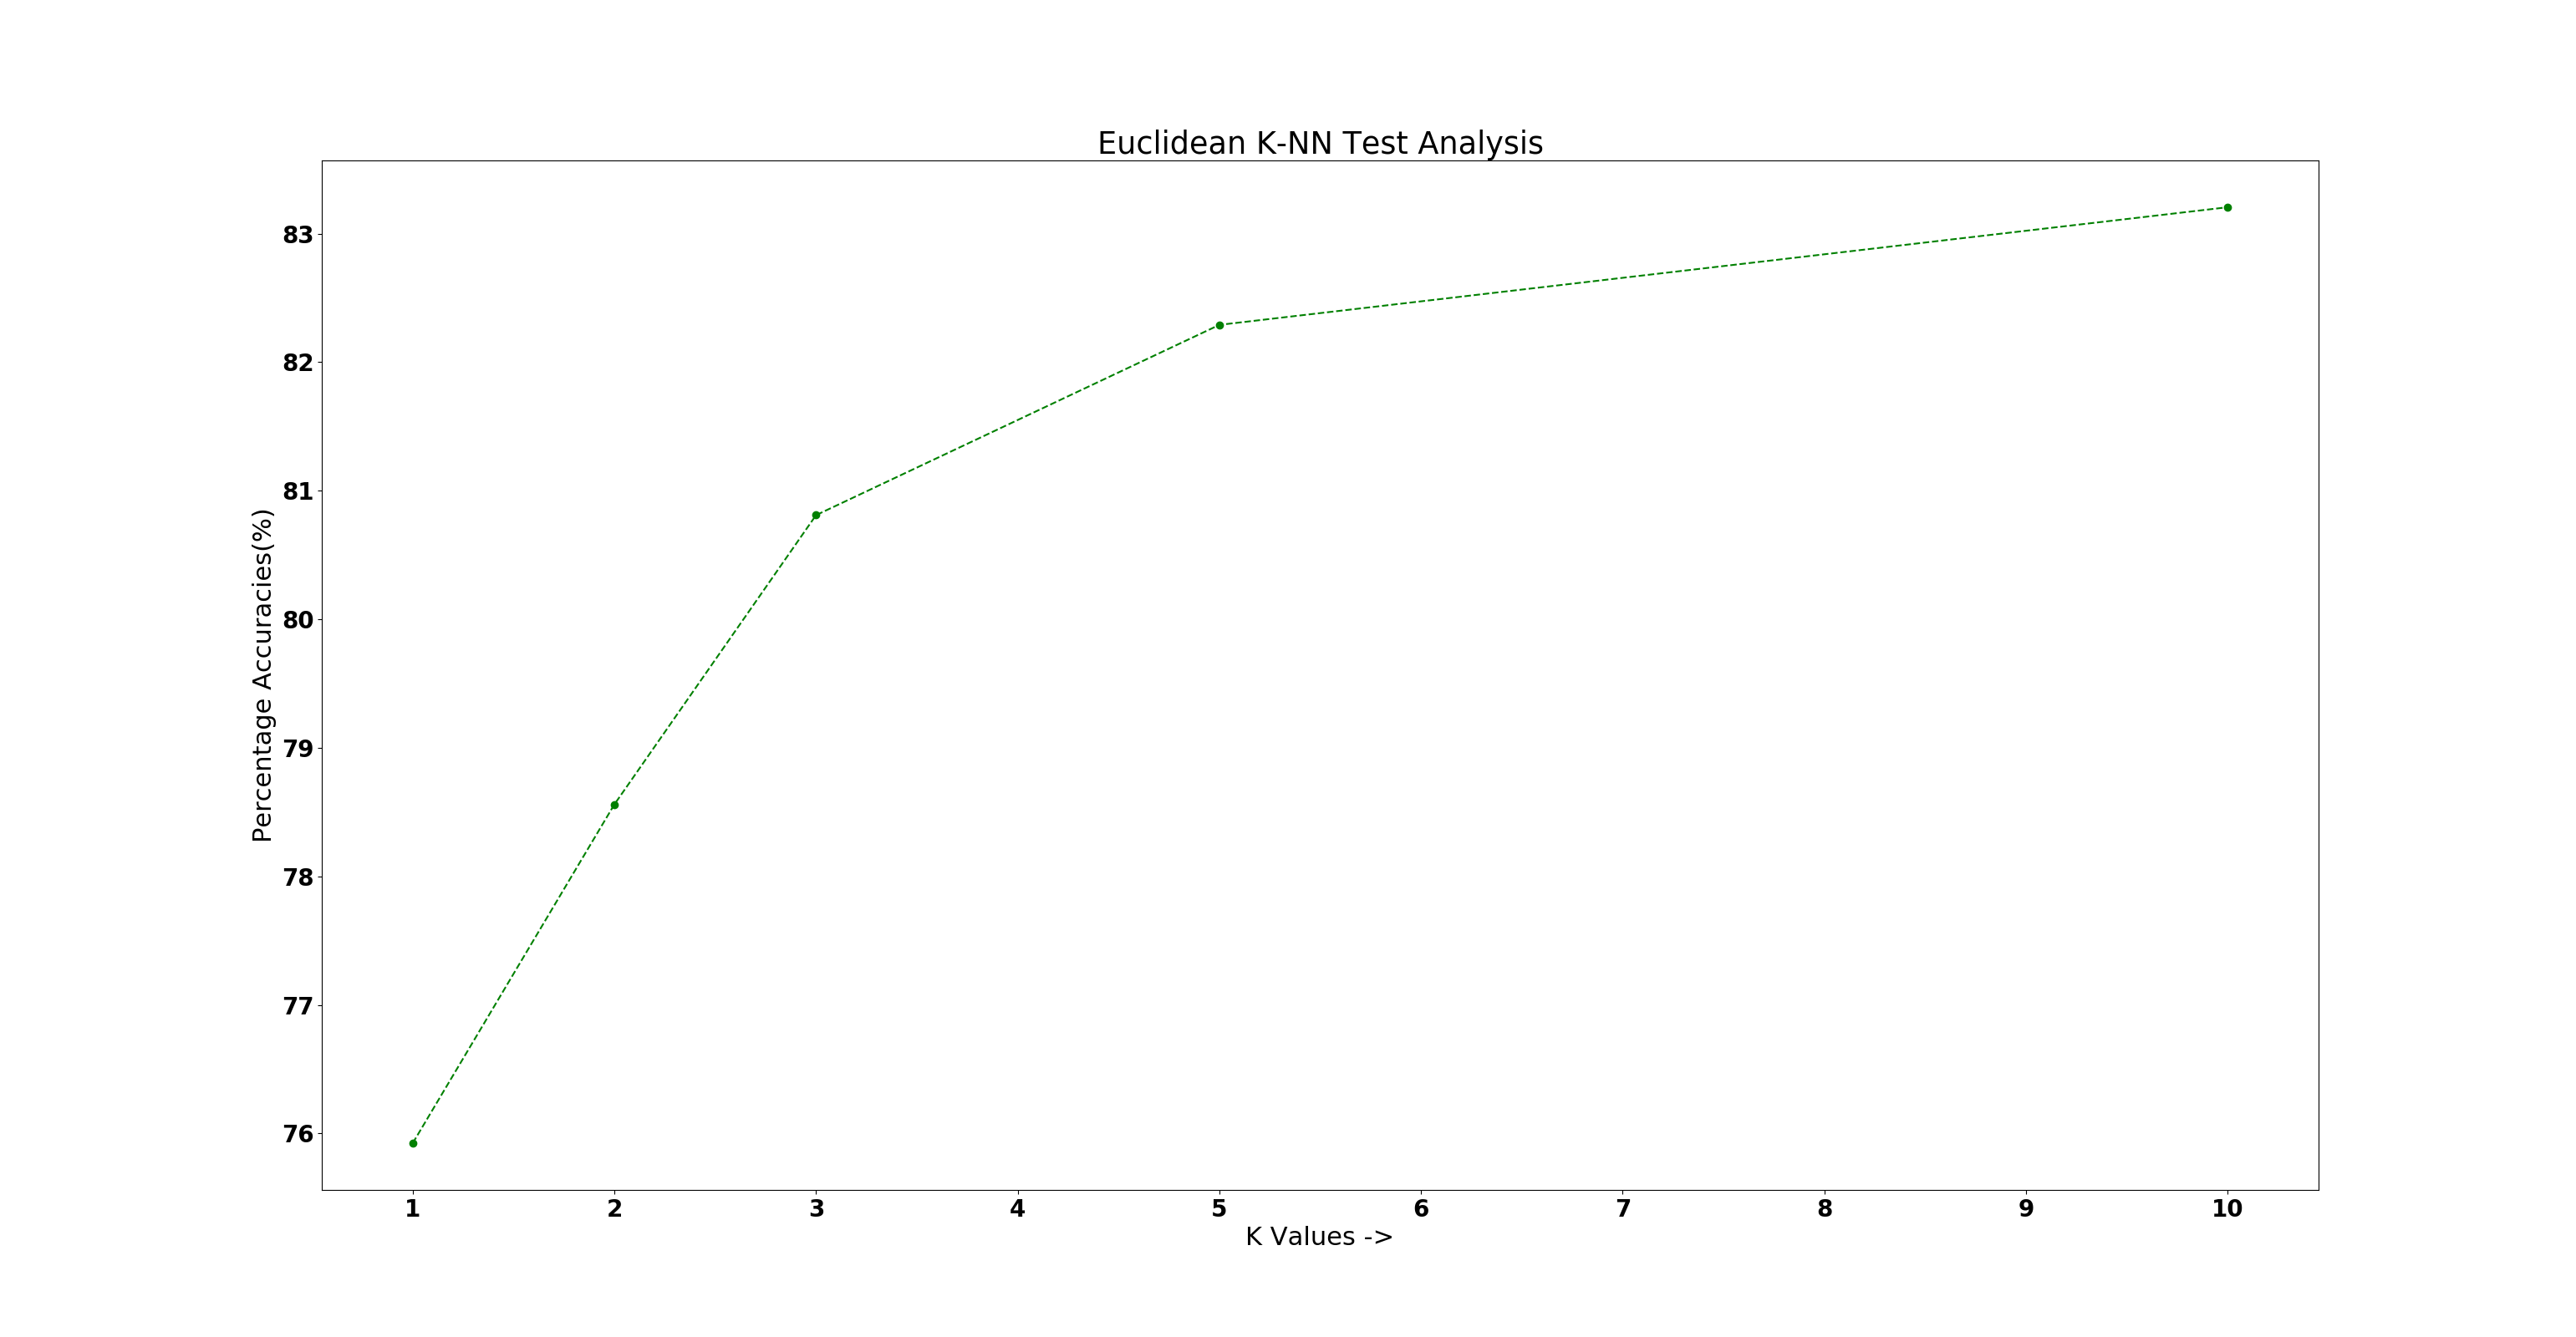
\includegraphics[width=1.2\columnwidth]{Q1_6_final.png}%
\caption{Graph depicting test set accuracies using Euclidean distance metric}%
\label{fig:proto}%
\end{figure}
We observe that as the value of k increases, the percentage accuracies keep increasing. Here are the precise values I obtained:
\begin{align}
    k = 1 &: 75.925 \% \\
    k = 2 &: 78.56 \% \\
    k = 3 &: 80.81 \% \\
    k = 5 &: 82.29 \% \\
    k = 10 &: 83.205 \% 
\end{align}
This can be attributed to the fact that increasing k helps in preventing over fitting. As the value of k increases, the areas assigned to each class become smoother, preventing the decision boundary from tailoring itself too much to training data. This improves the capability of the algorithm to generalise and hence the performance improves as k increases. \subsection*{Part2}
The validation technique used was held out validation. I took the training data from the train.dat file. Then I randomly shuffled the entire data and picked the first 40,000 training points for my Xtr and Ytr. The rest 20,000 data points acted as the cross validation points. The prediction was then done for the following values of k: 1,5,8,12,15,19,20.

On measuring the accuracies for each k, I realised that k=12 gave me the highest accuracy percentage.So ideally k=12 is the best value I obtain.But I soon realised that running LMNN for k=12 was not feasible. So, instead I observed that uptill k=5, the surge in accuracy was very high, after which, even though the percentage accuracies did improve, the increase was very little. So, I set k=5 as my choice of k for LMNN training.

\subsection*{Part3}
Using the above set value of k and choosing only 10,000 out of the 60,000 training points to train my LMNN model, I built the model and saved in the model.npy file. The decision to take 1/6 of the data was propelled by the fact that running LMNN for the entire dataset was not feasible on my machine.

The test accuracy obtained for the model thus learnt was 82.78 \%







\end{mlsolution}			
					
\end{document}